\headline{{\textbf{\Large\sffamily Growing Together:}}\\
          {\textbf{\large\sffamily Bonsai Club News}}}
\label{2025-03-news}

\topic{Save on Club Merchandise with Shared Order!}
\noindent
The club's merchandise can be found at \url{https://overrock.uk/product-category/tw-bonsai/}. If you're thinking of making a purchase soon, reach out to Brendan on WhatsApp. Placing a shared order could help save a little on shipping costs.

\medskip
\topic{Bonsai Resources at Your Fingertips}
\noindent  
Our bonsai club is proud to offer a wide range of resources to help you grow and thrive in your bonsai journey. All these resources are conveniently organized on our Discord channel. If you're a subscribed member and haven’t yet accessed the channel, simply \href{https://discord.gg/N6yka6XJ}{follow this link}.

Once you join, you'll land in the \href{https://discord.com/channels/873817545013071872/1118677826208550923}{welcome chat}. On the left\--hand side, you'll find a list of subchannels, each dedicated to a specific topic or service, such as \href{https://discord.com/channels/873817545013071872/1039691122148130876}{club payments}, \href{https://discord.com/channels/873817545013071872/1001189937409949698}{book recommendations}, and more. 

Whether you're a seasoned enthusiast or a new member, these resources are here to support your passion for bonsai. Don't miss out---get connected today!

\medskip	
\topic{Bonsai Insights: Information Pack for All Members}
\noindent
We've put together an information pack for all members of the club – from beginners to seasoned enthusiasts. This pack offers a wealth of resources, including access to a selection of our lockdown ZOOM talks featuring some of the best Bonsai artists in the country.

The following link will direct you to a Google slideshow \href{https://docs.google.com/presentation/d/1L5SRA_ZSvnGMLbRt0CSf-Uz7BaiOfxOs7OUHMM_XrTY/edit?usp=sharing}{New \& Existing Members Information Pack}, so feel free to explore it at your own pace. We recommend starting with Andy Hardman’s talk on tree biology (Video 1), where he delves into how trees function and what they need to thrive.

\medskip
\topic{Don't Leaf Us Hanging: Meetup Time!}
\noindent
Come join us at 7pm on \textbf{13th March 2025} in the bar area at \emph{Whitton Community Centre, Percy Road, Whitton TW2 6JL}. Branching out, the subject of next \textbf{Tree of the Month} display will be \textbf{Yamadori, urban or wild}---bring your best!
	
% \topic{TWBC Winter Show 2025!}
% \noindent
% Our first show of the year is fast approaching! Please come along early to help setup the display and help the organisation during the day. Thanks in advance! See you on \textbf{Sunday, 2nd February 2025} at \emph{St Richard Reynolds Catholic College, Clifden Road, Twickenham, TW1 4LT}! 
	
% \topic{Grafting Workshop – Express Interest Now!}
% \noindent
% Steve will lead a workshop in March on grafting \textbf{Paul's Scarlet Hawthorn} onto regular hawthorn rootstock. Plants will be provided (limited availability). The workshop will cost \textbf{£5} and take place during the March club night. Contact Steve via WhatsApp to secure your spot. 

\closearticle

\medskip
\begin{center}
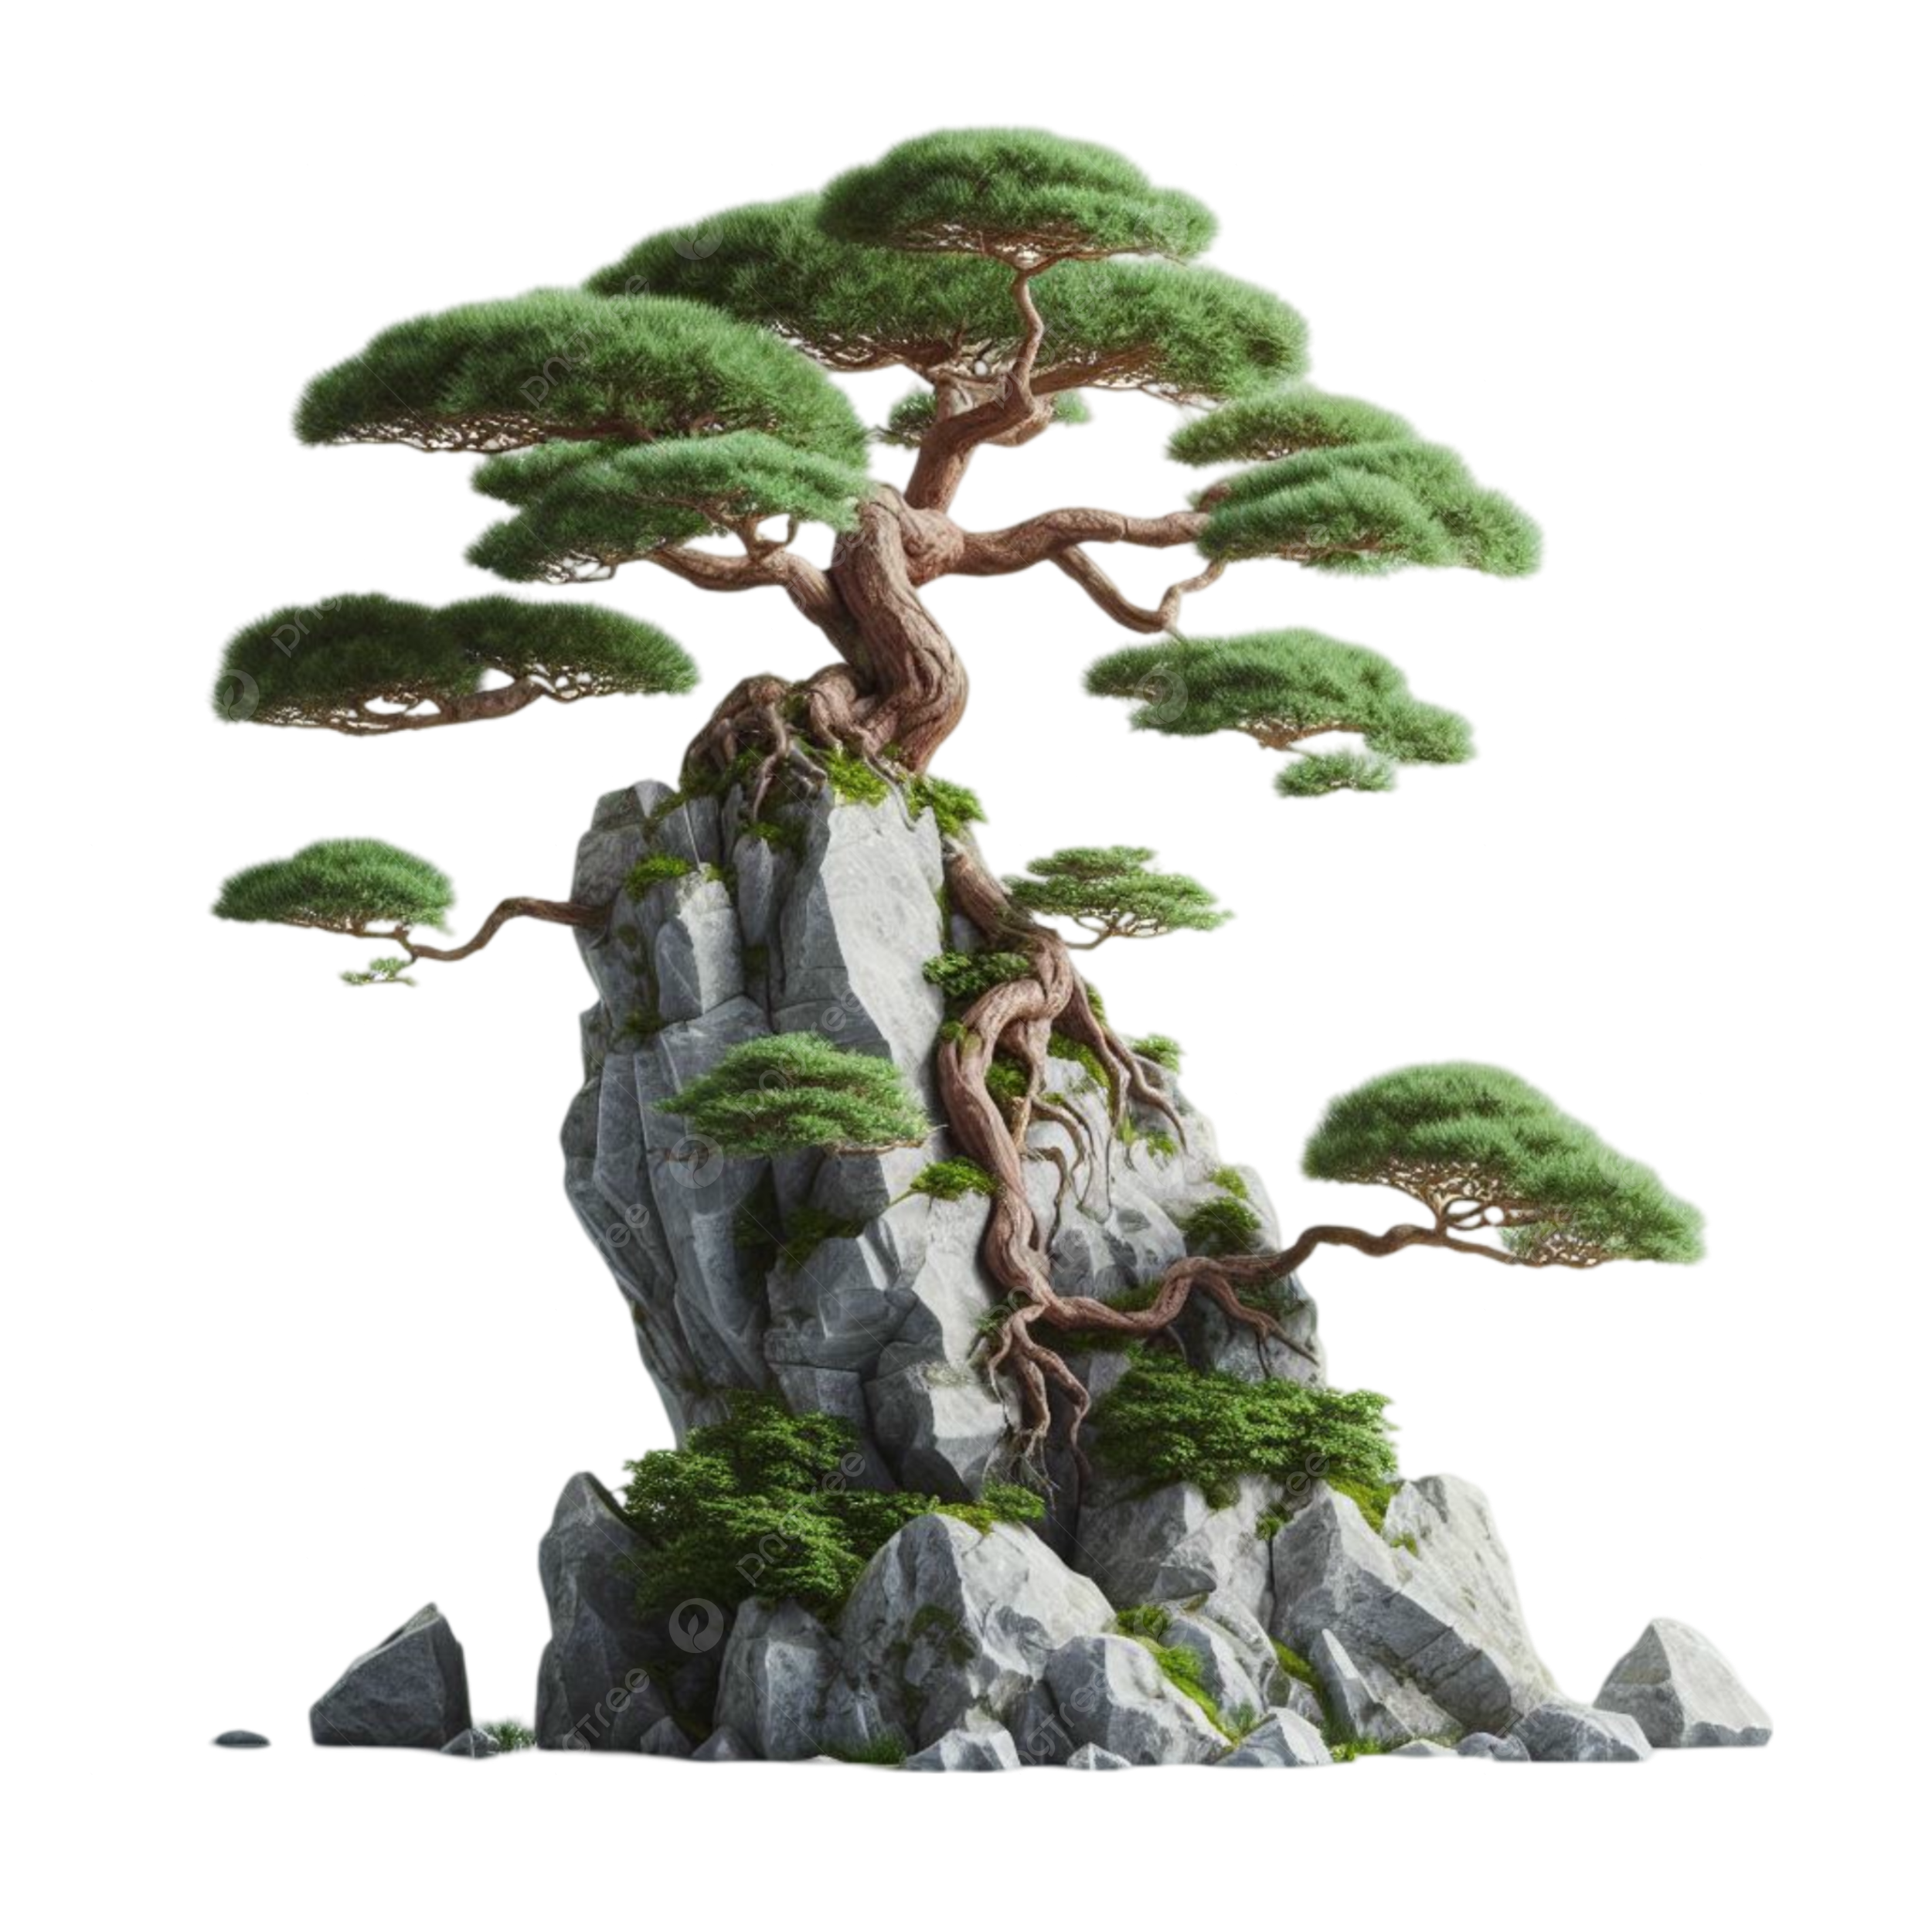
\includegraphics[width=0.5\columnwidth]{res/filler_d.png}
\end{center}

\columnbreak